\documentclass[11pt]{article}
%%%%%%%%%%%%%%%%%%%%%%%%%%%%%%%%%%%%%%%%%%%%%%%
% load packages 
% these are the set of packages that i typically use. we'll only discuss a few
% packages we will discuss
\usepackage{Sweave} % use sweave
\usepackage[top=.9in, bottom=.9in, left=.9in, right=.8in]{geometry} % set margins
\usepackage[pdfborder={0 0 0}]{hyperref}% For email addresses
  \hypersetup{ % make TOC clickable links
    colorlinks,
    citecolor=black,
    filecolor=black,
    linkcolor=blue,
    urlcolor=black
  }
\usepackage[draft]{fixme} % enable comments in the margins
  \fxsetup{layout=footnote, marginclue}
\usepackage{lineno,xcolor}% Running line numbers:
  \linenumbers
  \setlength\linenumbersep{5pt}
  \renewcommand\linenumberfont{\normalfont\tiny\sffamily\color{gray}}

% packages we won't discuss
\usepackage{fullpage}
\usepackage{float} 
\usepackage{enumerate}
\usepackage[utf8]{inputenc}
\usepackage{titling}
\usepackage{caption}
\usepackage{subcaption}
\setlength{\droptitle}{-4em} 
\usepackage{amsmath}
\usepackage{natbib} % unnumbered bibliography style
\usepackage{indentfirst} % indent first paragraph of a section
\usepackage{chngcntr} % for appendix figure counting
\usepackage{authblk}

% end load packages 
%%%%%%%%%%%%%%%%%%%%%%%%%%%%%%%%%%%%%%%%%%%%%%%

\begin{document} 

%%%%%%%%%%%%%%%%%%%%%%%%%%%%%%%%%%%%%%%%%%%%%%%
% Sweave Options

\DefineVerbatimEnvironment{Sinput}{Verbatim} {xleftmargin=0em}
\DefineVerbatimEnvironment{Soutput}{Verbatim}{xleftmargin=2em}
\DefineVerbatimEnvironment{Scode}{Verbatim}{xleftmargin=0em}
\fvset{listparameters={\setlength{\topsep}{0pt}}}
\renewenvironment{Schunk}{\vspace{\topsep}}{\vspace{\topsep}}
% the next 5 lines eliminate all the spaces in my basic version of the documents, but not in the master file
\newlength{\fancyvrbtopsep}
\newlength{\fancyvrbpartopsep}
\makeatletter
\FV@AddToHook{\FV@ListParameterHook}{\topsep=\fancyvrbtopsep\partopsep=\fancyvrbpartopsep}
\makeatother
% End Sweave options
%%%%%%%%%%%%%%%%%%%%%%%%%%%%%%%%%%%%%%%%%%%%%%%


\title{Appendix A: A simple IPM for a long-lived perennial plant}
\author{Cory Merow, Johan P. Dahlgren, C.J.E. Metcalf,\\ Dylan Z. Childs, M.E.K. Evans, Eelke Jongejans, Sydne Record,\\ Mark Rees, Roberto Salguero-Gomez \& Sean M. McMahon}
\maketitle
\tableofcontents

% Stangle('/Users/ctg/Dropbox/Shared/IPM_guide/Appendices/Appendix_A_Simple\ _IPM_Cory/files_for_rnw/IPM_guide_appendix_A.Rnw')
\textbf{Contact: Cory Merow (cory.merow@gmail.com)}



%%%%%%%%%%%%%%%%%%%%%%%%%%%%%%%%%%%%%%%%%%%%%%%%%%%%%%%%%%%%%%%
%%%%%%%%%%%%%%%%%%%%%%%%%%%%%%%%%%%%%%%%%%%%%%%%%%%%%%%%%%%%%%%

\section*{Abstract}
Integral Projection Models (IPMs) use vital rate regressions to parameterize transition kernels that can be used for population projections. Here, we introduce an extremely simple IPM for a the long-live alpine perennial plant \emph{Dracocephalum austriacum}. The analyses minimize the complexity of the R code in order to make the model transparent. After building a basic model, we illustrate ways to improve it, including, comparing alternative growth models, non-constant variance in growth, including a model for flowering probability. We calculate basic population statistics, including population growth rate, sensitivity, elasticity, and passage times throughout to check the plausibility of the model. We also illustrate a series of diagnostics, including correcting for eviction, determining asymptotic maximum size, and exploring the importance of transient dynamics. The model is associated with Example 1, Section II.A. in the main text.

\newpage

%%%%%%%%%%%%%%%%%%%%%%%%%%%%%%%%%%%%%%%%%%%%%%%%%%%%%%%%%%%%%%%%%%%%%%%%%%%%%%
%%%%%%%%%%%%%%%%%%%%%%%%%%%%%%%%%%%%%%%%%%%%%%%%%%%%%%%%%%%%%%%%%%%%%%%%%%%%%%

\section{Introduction}
\label{sec:Introduction}
In this appendix, we illustrate how to build an IPM 'from scratch.' We begin with a simulated data set, build vital rate regressions, combine these regressions into an IPM kernel, and perform basic analyses of asymptotic dynamics. We begin with the simplest model of a perennial plant (corresponding to Example 1 in the main text) that one might consider for an IPM and iteratively improve the model to simulate the process by which a researcher might develop an IPM.

%Note that to extract just the R code from this document, in R you can type \\ \texttt{Stangle("IPM\_guide\_appendix\_A.Rnw")}. This links to the Sweave file, not the pdf that you are currently reading, and will produce a file named \texttt{"IPM\_guide\_appendix\_A.R"} in your current working directory (use \texttt{getwd()} to figure out what that is).

%%%%%%%%%%%%%%%%%%%%%%%%%%%%%%%%%%%%%%%%%%%%%%%%%%%%%%%%%%%%%%%%%%%%%%%%%%%%%%
%%%%%%%%%%%%%%%%%%%%%%%%%%%%%%%%%%%%%%%%%%%%%%%%%%%%%%%%%%%%%%%%%%%%%%%%%%%%%%

\section{Study system/objectives}
\label{sec:Study system/objectives}

The goal of this exercise is to illustrate how to perform basic IPM analyses of asymptotic population growth rate, stable stage structure, reproductive values, sensitivities and elasticities of population growth rate to matrix elements. We then develop improvements to the model and illustrate the various diagnostics discussed in the main text to illustrate the iterative process of moving between data, models, and predictions to produce a biologically robust IPM. The data are simulated to clearly illustrate some of the subtle patterns we extract with the models, however the simulations derive from a model for a single annual transition (2001-2002) of the alpine plant \emph{Dracocephalum austriacum}. Nicole et al. (2011) describe \emph{Dracocephalum austriacum} as follows (see references therein):

\emph{`The Austrian Dragonhead (D. austriacum L., Lamiaceae) is a long-lived perennial plant occurring from the Pyrenees to the Caucasus, with scattered populations in Western Europe (Bensettiti et al. 2002). The plant is 20 to 50 cm high, with hairy stems and large blue–violet insect-pollinated flowers (3.5 to 5 cm in length). Dracocephalum austriacum does not spread clonally and seeds lack adaptations for dispersal. It usually occurs in habitat patches where competition with other plants is low and competition with shrubs and trees may have a negative effect on performance (Olivier et al. 1995). Dracocephalum austriacum is listed as Vulnerable by the World Conservation Union (IUCN) and is protected under National, European and international legislation (Red List of French Endangered Flora, Habitats Directive, Bern Convention). Threats include pillaging, trampling and damage by grazing cattle (Bensettiti et al. 2002). Previous studies with this species have shown large population differences in adaptive genetic variation (Bonin et al. 2007) and positive correlations between population heterozygosity and stochastic population growth rate (Nicole 2005). The present field study was carried out in 7 of the 15 known French populations of D. austriacum. The study populations occur in the subalpine zone (1250 to 2000 m a.s.l.) of the Alps, on exposed, xeric, stony grasslands or heaths, preferentially on calcareous, thin soils (Lauber and Wagner 1998). Populations vary widely in size, density, habitat characteristics and soil composition.'}

%%%%%%%%%%%%%%%%%%%%%%%%%%%%%%%%%%%%%%%%%%%%%%%%%%%%%%%%%%%%%%%%%%%%%%%%%%%%%%
%%%%%%%%%%%%%%%%%%%%%%%%%%%%%%%%%%%%%%%%%%%%%%%%%%%%%%%%%%%%%%%%%%%%%%%%%%%%%%

\section{Data}
\label{sec:Data}

We begin with reading in data. You'll have to set your own file path here. The data is in a .csv file included in the Supplementary Materials.

\begin{Schunk}
\begin{Sinput}
 d <- read.csv('Appendix_A_Simple_data.csv')
\end{Sinput}
\end{Schunk}

You will notice that adults are stored at the beginning of the data set with values for size (measured in 2001) and sizeNext (measured in 2002). The number of seeds (fec.seed) and flowering status (fec.flower) were measured in 2001.
\begin{Schunk}
\begin{Sinput}
 head(d)
\end{Sinput}
\begin{Soutput}
  size sizeNext surv fec.seed fec.flower
1 3.09       NA    0       NA         NA
2 2.81       NA    0       NA         NA
3 4.46     6.07    1       15          1
4 1.68       NA    0       NA         NA
5 3.99       NA    0       NA         NA
6 4.07       NA    0       NA         NA
\end{Soutput}
\end{Schunk}

New recruits are stored at the end of the data frame and were only observed in the second survey (2002).

\begin{Schunk}
\begin{Sinput}
 tail(d)
\end{Sinput}
\begin{Soutput}
    size sizeNext surv fec.seed fec.flower
495   NA     1.78   NA       NA         NA
496   NA     1.01   NA       NA         NA
497   NA     1.68   NA       NA         NA
498   NA     1.44   NA       NA         NA
499   NA     1.08   NA       NA         NA
500   NA     1.62   NA       NA         NA
\end{Soutput}
\end{Schunk}

Note that we use NAs for missing or non-applicable data rather than 0 or some other indicator because this causes them to be automatically excluded from R's regression functions. For example, an individual that doesn't survive cannot grow or reproduce, hence values for sizeNext, fec.seed, and fec.flower are NA.
%%%%%%%%%%%%%%%%%%%%%%%%%%%%%%%%%%%%%%%%%%%%%%%%%%%%%%%%%%%%%%%%%%%%%%%%%%%%%%
%%%%%%%%%%%%%%%%%%%%%%%%%%%%%%%%%%%%%%%%%%%%%%%%%%%%%%%%%%%%%%%%%%%%%%%%%%%%%%

\section{Analysis}
\label{sec:Analysis}

\subsection{Plots for data exploration}
\label{sec:Plots for data exploration}
  
The model used here is described in detail in Example 1 in Section II of the main text. Using the notation there, this model can be written as:

\begin{equation}
n_{t+1}(z')=\int_\Omega \ K(z) n_{t}(z) dz =\int_\Omega \ [P(z',z) + F(z',z)] n_{t}(z) dz
\end{equation}

\begin{equation}
P(z',z) = s(z)\ g(z',z) 
\end{equation}

\begin{equation}
F(z',z) = p_{flower}(z)\ f_{seeds}(z)\ p_{estab}\ f_{recruit size}(z’)
\end{equation}

To understand the data, we plot survival, growth/shrinkage/stasis, number of seeds, and size of recruits as a function of our state variable, size.   

\begin{figure}[H]
\begin{center}
\begin{Schunk}
\begin{Sinput}
     par(mfrow=c(2,2),mar=c(4,4,2,1)) 
     plot(d$size,jitter(d$surv),xlab="Size (t)", ylab="Survival to t+1") # jittered 
     plot(d$size,d$sizeNext,xlab="Size (t)",ylab="Size (t+1)")  
     plot(d$size,d$fec.seed,xlab="Size (t)",ylab="Seed Number") 
     hist(d$sizeNext[is.na(d$size)],main='',xlab='Recruit Size')
\end{Sinput}
\end{Schunk}
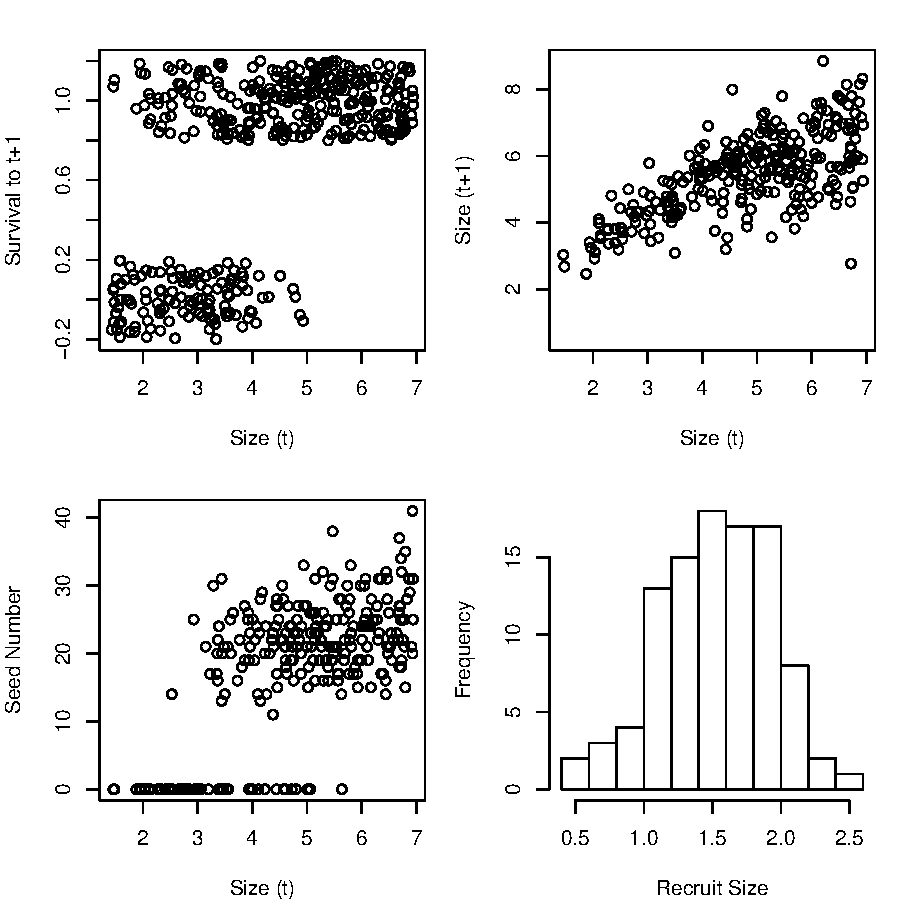
\includegraphics{IPM_Guide_Appendix_A-fig1}

\caption{Exploration of vital rate data.}
\label{fig:figA1}
\end{center}
\end{figure}


%%%%%%%%%%%%%%%%%%%%%%%%%%%%%%%%%%%%%%%%%%%%%%%%%%%%%%%%%%%%%%%%%%%%%%%%%%%%%%
%%%%%%%%%%%%%%%%%%%%%%%%%%%%%%%%%%%%%%%%%%%%%%%%%%%%%%%%%%%%%%%%%%%%%%%%%%%%%%

\subsection{Build regressions for vital rate functions}
\label{sec:Build regressions for vital rate functions}

We begin by setting up a data frame of the model parameters. These parameters will be estimated and recorded below.
\begin{Schunk}
\begin{Sinput}
 params=data.frame(
    surv.int=NA,          # Intercept from logistic regression of survival 
    surv.slope=NA,        # Slope from logistic regression of survival 
    growth.int=NA,        # Intercept from linear regression of growth
    growth.slope=NA,      # Slope from linear regression of growth
    growth.sd=NA,         # Residual sd from the linear regression of growth
    seed.int=NA,          # Intercept from Poisson regression of seed number
    seed.slope=NA,        # Slope from Poisson regression of seed number
    recruit.size.mean=NA, # Mean recruit size
    recruit.size.sd=NA,   # Standard deviation of recruit size
    establishment.prob=NA # Probability of establishment
  )
\end{Sinput}
\end{Schunk}
Next, we build each of the vital rate regressions and store the coefficients.
\begin{Schunk}
\begin{Sinput}
 # 1. survival: logistic regression
 surv.reg=glm(surv~size,data=d,family=binomial())
 summary(surv.reg)
\end{Sinput}
\begin{Soutput}
Call:
glm(formula = surv ~ size, family = binomial(), data = d)

Deviance Residuals: 
    Min       1Q   Median       3Q      Max  
-2.2275  -0.5815   0.2491   0.5597   2.0972  

Coefficients:
            Estimate Std. Error z value Pr(>|z|)    
(Intercept)  -3.9646     0.4760  -8.329   <2e-16 ***
size          1.2897     0.1338   9.642   <2e-16 ***
---
Signif. codes:  
0 ‘***’ 0.001 ‘**’ 0.01 ‘*’ 0.05 ‘.’ 0.1 ‘ ’ 1

(Dispersion parameter for binomial family taken to be 1)

    Null deviance: 488.69  on 399  degrees of freedom
Residual deviance: 315.82  on 398  degrees of freedom
  (100 observations deleted due to missingness)
AIC: 319.82

Number of Fisher Scoring iterations: 5
\end{Soutput}
\begin{Sinput}
 params$surv.int=coefficients(surv.reg)[1]
 params$surv.slope=coefficients(surv.reg)[2]
 # 2. growth: linear regression
 growth.reg=lm(sizeNext~size,data=d)
 summary(growth.reg)
\end{Sinput}
\begin{Soutput}
Call:
lm(formula = sizeNext ~ size, data = d)

Residuals:
    Min      1Q  Median      3Q     Max 
-3.8037 -0.5434  0.0932  0.5741  2.6732 

Coefficients:
            Estimate Std. Error t value Pr(>|t|)    
(Intercept)  2.68135    0.19580   13.69   <2e-16 ***
size         0.57922    0.03902   14.84   <2e-16 ***
---
Signif. codes:  
0 ‘***’ 0.001 ‘**’ 0.01 ‘*’ 0.05 ‘.’ 0.1 ‘ ’ 1

Residual standard error: 0.8866 on 278 degrees of freedom
  (220 observations deleted due to missingness)
Multiple R-squared:  0.4421,	Adjusted R-squared:  0.4401 
F-statistic: 220.3 on 1 and 278 DF,  p-value: < 2.2e-16
\end{Soutput}
\begin{Sinput}
 params$growth.int=coefficients(growth.reg)[1]
 params$growth.slope=coefficients(growth.reg)[2]
 params$growth.sd=sd(resid(growth.reg))
\end{Sinput}
\end{Schunk}
  
For fecundity, note that we are pooling all individuals into this regression regardless of whether they flowered or not. A later exercise will be to explicitly model flowering probability, which necessary to deal with the many zeros that are observed in the plot for seed number in Fig. ~\ref{fig:figA1}.

\begin{Schunk}
\begin{Sinput}
 # 3. seeds: Poisson regression
 seed.reg=glm(fec.seed~size,data=d,family=poisson())
 summary(seed.reg)
\end{Sinput}
\begin{Soutput}
Call:
glm(formula = fec.seed ~ size, family = poisson(), data = d)

Deviance Residuals: 
    Min       1Q   Median       3Q      Max  
-6.5338  -1.8830   0.0529   1.5375   4.9690  

Coefficients:
            Estimate Std. Error z value Pr(>|z|)    
(Intercept)  1.33234    0.06370   20.92   <2e-16 ***
size         0.30647    0.01164   26.34   <2e-16 ***
---
Signif. codes:  
0 ‘***’ 0.001 ‘**’ 0.01 ‘*’ 0.05 ‘.’ 0.1 ‘ ’ 1

(Dispersion parameter for poisson family taken to be 1)

    Null deviance: 2598.3  on 279  degrees of freedom
Residual deviance: 1840.1  on 278  degrees of freedom
  (220 observations deleted due to missingness)
AIC: 2942.2

Number of Fisher Scoring iterations: 5
\end{Soutput}
\begin{Sinput}
 params$seed.int=coefficients(seed.reg)[1]
 params$seed.slope=coefficients(seed.reg)[2]
\end{Sinput}
\end{Schunk}
In the data frame, recruits are those individuals who have a value for sizeNext but not for size. We simply take the mean and standard deviation of their size for use in a normal distribution. We assume that offspring size is independent of maternal size so we only need to describe the distribution of offspring sizes in terms of its mean and variance.
\begin{Schunk}
\begin{Sinput}
 # 4. size distribution of recruits
 params$recruit.size.mean=mean(d$sizeNext[is.na(d$size)])
 params$recruit.size.sd=sd(d$sizeNext[is.na(d$size)])
\end{Sinput}
\end{Schunk}

These data represent a single year's worth of data, hence establishment probability can be estimated by dividing the number of observed recruits by the number of seeds. the growth/survival measurements were taken in year t whereas the recruit sizes were measured in year t+1. Importantly, this calculation ignores all the processes that might lead to seed loss, however we make this assumption for the sake of simplicity in our illustration.
\begin{Schunk}
\begin{Sinput}
 # 5. establishment probability
 params$establishment.prob=sum(is.na(d$size))/sum(d$fec.seed,na.rm=TRUE)
\end{Sinput}
\end{Schunk}

Now, compare each of the vital rate models (red lines) to the data in Fig. ~\ref{fig:figA2}.

Note that in practice, it is critical to check how well the vital rate models describe the data. Model selection is really the most important step in building an IPM because all inference derives from the quality of these regressions. Issues of model selection are discussed in the Section III.A of the main text and Appendix D. 

\begin{figure}[H]
\begin{center}
\begin{Schunk}
\begin{Sinput}
     par(mfrow=c(2,2))
     xx=seq(0,8,by=.01) # sizes at which to evaluate predictions
     plot(d$size,jitter(d$surv), xlab="Size (t)",ylab="Survival to t+1") # jittered 
     lines(xx,predict(surv.reg,
        data.frame(size=xx),type='response'), col='red',lwd=3)
     plot(d$size,d$sizeNext,xlab="Size (t)",ylab="Size (t+1)")  
     lines(xx,predict(growth.reg,data.frame(size=xx)),col='red',lwd=3)
     plot(d$size,d$fec.seed,xlab="Size (t)",ylab="Seed Number (t)")
     lines(xx,predict(seed.reg,
        data.frame(size=xx),type='response'),col='red',lwd=3)
     hist(d$sizeNext[is.na(d$size)],freq=FALSE,xlab="Recruit size",main='')
     lines(xx,dnorm(xx,params$recruit.size.mean,
        params$recruit.size.sd), col='red',lwd=3)
\end{Sinput}
\end{Schunk}
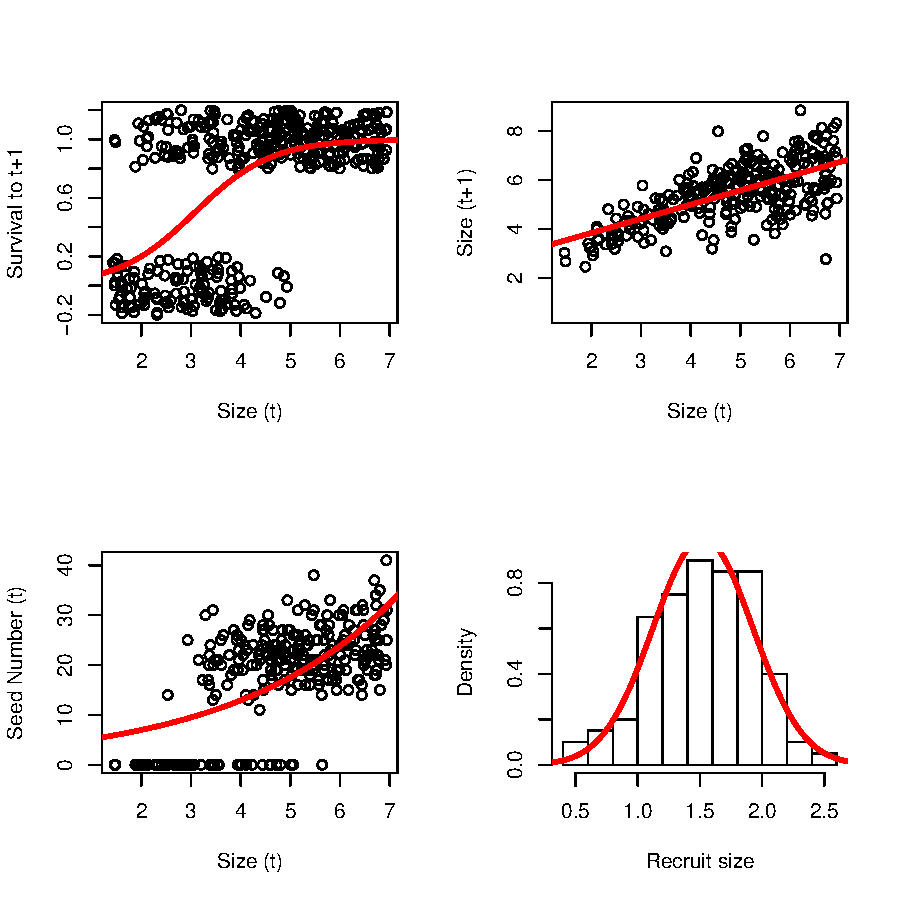
\includegraphics{IPM_Guide_Appendix_A-fig2}
\caption{Compare vital rate regressions to data.}
\label{fig:figA2}
\end{center}
\end{figure}

%%%%%%%%%%%%%%%%%%%%%%%%%%%%%%%%%%%%%%%%%%%%%%%%%%%%%%%%%%%%%%%%%%%%%%%%%%%%%%
%%%%%%%%%%%%%%%%%%%%%%%%%%%%%%%%%%%%%%%%%%%%%%%%%%%%%%%%%%%%%%%%%%%%%%%%%%%%%%


\subsection{Define functions to describe life history}
\label{sec:Define functions to describe life history}

Each of the functions below represents one or more of the vital rates. These functions are used to build the IPM using output (the coefficients) from the regressions developed above. 
  
These functions represent the modeler's decision about how to decompose the life cycle. In this very simple example, we model (1) survival, (2) growth, (3) seed number, (4) the seedling size distribution and (5) the establishment probability. In practice, we'd need to decide what regressions to build in part B in advance, but it's easier to digest this section after you've seen the regressions above, so fortunately we built all the right regressions already. In practice, sections 1.4.2 and 1.4.3 are iterative should inform one another. For example, the level of detail included in the life history models can be determined by the data availability and quality of the candidate vital rate regressions.
  
% TODO: could talk through these functions
\begin{Schunk}
\begin{Sinput}
   # 1. survival probability function
 s.x=function(x,params) {
    u=exp(params$surv.int+params$surv.slope*x)
    return(u/(1+u))
  }
 # 2. growth function
 g.yx=function(xp,x,params) { 			
    dnorm(xp,mean=params$growth.int+params$growth.slope*x,sd=params$growth.sd)
  }
 # 3. reproduction function      
 f.yx=function(xp,x,params) { 		
    params$establishment.prob*
      dnorm(xp,mean=params$recruit.size.mean,sd=params$recruit.size.sd)*
      exp(params$seed.int+params$seed.slope*x)
  }
\end{Sinput}
\end{Schunk}

%%%%%%%%%%%%%%%%%%%%%%%%%%%%%%%%%%%%%%%%%%%%%%%%%%%%%%%%%%%%%%%%%%%%%%%%%%%%%%
%%%%%%%%%%%%%%%%%%%%%%%%%%%%%%%%%%%%%%%%%%%%%%%%%%%%%%%%%%%%%%%%%%%%%%%%%%%%%%

\subsection{Make a kernel}
\label{sec:Make_a_kernel}
In this section, we combine the vital rate functions to build the discretized IPM kernel, which we'll call the IPM matrix (e.g. shown in Fig. 2c in the main text).These steps are performed behind the scenes in the IPMpack package used in Appendices C-G for convenience, but we show them here for illustrative purposes. To integrate, we begin by defining the boundary points (b; the edges of the cells defining the matrix), mesh points (y; the centers of the cells defining the matrix and the points at which the matrix is evaluated for the midpoint rule of numerical integration), and step size (h; the widths of the cells). The integration limits (min.size and max.size) span the range of sizes observed in the data set, and then some.

\begin{Schunk}
\begin{Sinput}
 min.size=.9*min(c(d$size,d$sizeNext),na.rm=T)
 max.size=1.1*max(c(d$size,d$sizeNext),na.rm=T)
 n=100 # number of cells in the matrix
 b=min.size+c(0:n)*(max.size-min.size)/n # boundary points  
 y=0.5*(b[1:n]+b[2:(n+1)]) # mesh points
 h=y[2]-y[1] # step size
\end{Sinput}
\end{Schunk}

Next, we make the IPM matrices. The function outer() evaluates the matrix at all pairwise combinations of the two vectors y and y and returns matrices representing the kernel components for growth and fecundity, respectively. For the numerical integration, we're using the midpoint rule (the simplest option) estimate the area under a curve. The midpoint rule assumes a rectangular approximation. The heights of the rectangles are given by the outer function and the width of the rectangles is h. 
%TODO could explain more
\begin{Schunk}
\begin{Sinput}
 G=h*outer(y,y,g.yx,params=params) # growth matrix
 S=s.x(y,params=params)            # survival 
 F=h*outer(y,y,f.yx,params=params) # reproduction matrix
 P=G                               # placeholder; redefine P on the next line
 for(i in 1:n) P[,i]=G[,i]*S[i]    # growth/survival matrix
 K=P+F                             # full matrix
\end{Sinput}
\end{Schunk}

The result is 100 x 100 cell discretization of the kernel, \emph{K}. For analyses, we can now apply the tools for matrix projection models (cf. Caswell 2001) to \emph{K}.

\subsection{Basic analyses}
\label{sec:Basic analyses}
Analyses usually begin with obtaining the eigenvalues ($\lambda$) and eigenvectors (v-left; w-right) of the matrix. These are useful for understanding the asymptotic dynamics. The dominant eigenvalue gives the asymptotic population growth rate (lam). The right eigenvector gives the stable stage distribution and the left eigenvector gives the reproductive value, when normalized.
\begin{Schunk}
\begin{Sinput}
 (lam <- Re(eigen(K)$values[1]))
\end{Sinput}
\begin{Soutput}
[1] 1.013391
\end{Soutput}
\begin{Sinput}
 w.eigen <- Re(eigen(K)$vectors[,1])
 stable.dist <- w.eigen/sum(w.eigen) 
 v.eigen <- Re(eigen(t(K))$vectors[,1])
 repro.val <- v.eigen/v.eigen[1] 
\end{Sinput}
\end{Schunk}
The eigen-things can be combined to obtain the sensitivity and elasticity matrices.
% TODO could define elas and sens
\begin{Schunk}
\begin{Sinput}
 v.dot.w=sum(stable.dist*repro.val)*h
 sens=outer(repro.val,stable.dist)/v.dot.w
 elas=matrix(as.vector(sens)*as.vector(K)/lam,nrow=n)
\end{Sinput}
\end{Schunk}
Finally, we plot these results  (stable size distribution, reproductive values, elasticity, sensitivity). 

\begin{figure}[H]
\begin{center}
\begin{Schunk}
\begin{Sinput}
     par(mfrow=c(2,3),mar=c(4,5,2,2)) 
     image.plot(y,y,t(K), xlab="Size (t)",ylab="Size (t+1)",
        col=topo.colors(100), main="IPM matrix")
     contour(y,y,t(K), add = TRUE, drawlabels = TRUE)
     plot(y,stable.dist,xlab="Size",type="l",main="Stable size distribution")
     plot(y,repro.val,xlab="Size",type="l",main="Reproductive values") 
     image.plot(y,y,t(elas),xlab="Size (t)",ylab="Size (t+1)",main="Elasticity")
     image.plot(y,y,t(sens),xlab="Size (t)",ylab="Size (t+1)", main="Sensitivity")
\end{Sinput}
\end{Schunk}
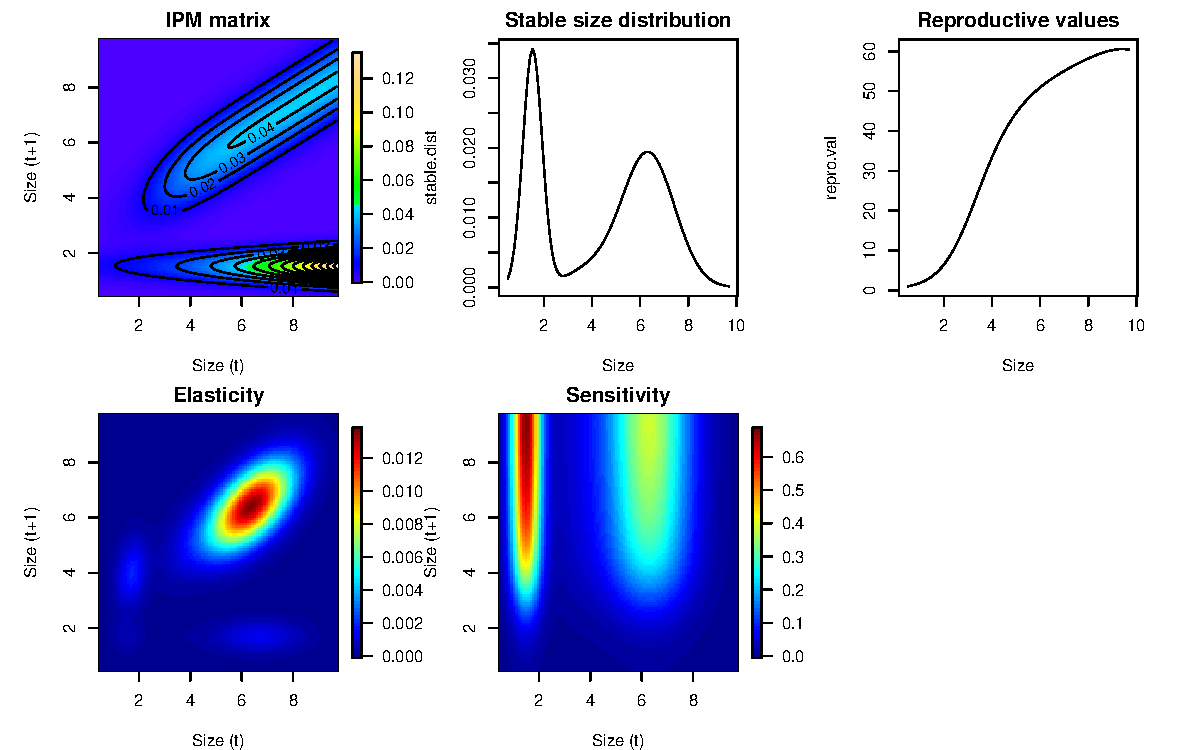
\includegraphics{IPM_Guide_Appendix_A-fig3}
\caption{Basic model output}
\label{fig:figA3}
\end{center}
\end{figure}

% TODO walk through interpretation

%%%%%%%%%%%%%%%%%%%%%%%%%%%%%%%%%%%%%%%%%%%%%%%%%%%%%%%%%%%%%%%%%%%%%%%%%%%%%%
%%%%%%%%%%%%%%%%%%%%%%%%%%%%%%%%%%%%%%%%%%%%%%%%%%%%%%%%%%%%%%%%%%%%%%%%%%%%%%

\subsection{Improving the model}
Typically, the workflow for building IPMs is iterative; based on preliminary analyses, we determine which important factors are missing or superfluous in the models. In this section, we make three improvements to the model built thus far: (1) we make the variance in growth among individuals a function of size (i.e. growth is more variable in larger individuals); (2) add a quadratic term for size to the growth function to capture the plateauing pattern in the growth data (Fig. 2b); (3) modify the fecundity function to include flowering probability, thereby recognizing that not all individuals reproduce.

%%%%%%%%%%%%%%%%%%%%%%%%%%%%%%%%%%%%%%%%%%%%%%%%%%%%%%%%%%%%%%%%%%%%%%%%%%%%%%
%%%%%%%%%%%%%%%%%%%%%%%%%%%%%%%%%%%%%%%%%%%%%%%%%%%%%%%%%%%%%%%%%%%%%%%%%%%%%%

\subsubsection{Size Dependent Variance in Growth}
\label{subsec:Size Dependent Variance in Growth}

First, we make the variance of the growth regression a function of size and obtain the value of $\lambda$. In the model above, we simply modeled the variance as constant, as seen in params\$growth.sd. By looking at the growth data in figure 1b you might guess that the variance increases as a function of size. You can see this in the following plot, where we plot the absolute value of the residuals of the growth regression against size.

\begin{figure}[H]
\begin{center}
\begin{Schunk}
\begin{Sinput}
   plot(growth.reg$model$size,abs(resid(growth.reg)),
      xlab='size',ylab='residual')
\end{Sinput}
\end{Schunk}
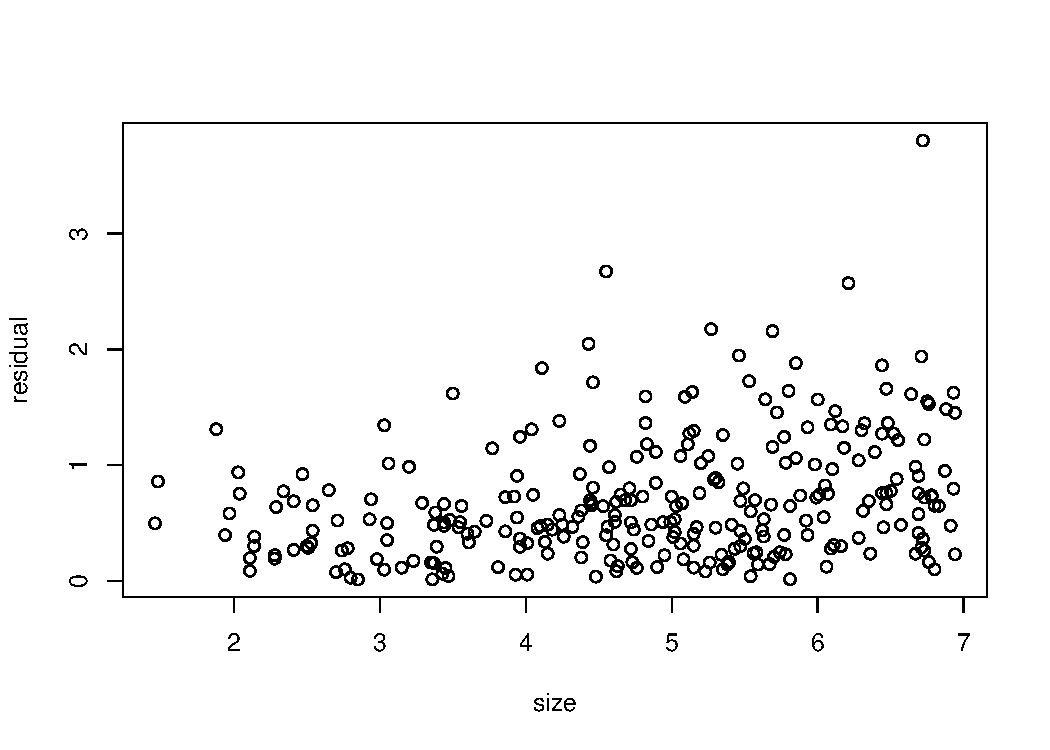
\includegraphics{IPM_Guide_Appendix_A-fig4}
\caption{Increasing variance in growth}
\label{fig:figA4}
\end{center}
\end{figure}

Incorporating nonuniform variance in the size distribution requires four  steps:

\begin{enumerate}[(A)]

\item Build a regression on the residuals of the growth regression as a function of size. This is most easily done using generalized least squares (GLS). GLS allows us to simultaneously fit a model for the expected size at t+1 and the variance. For this example, we'll model the variance in growth as an exponential function: $\sigma^2(size)=\sigma^2 exp[2*constant*size]$. See ?varExp for more details. The GLS model will estimate $\sigma^2$ and the constant, in addition to the intercept and slope used in the mean of the growth regression. gls() is in the nlme package, which you may need to install and load using install.packages('nlme') and library(nlme).

\begin{Schunk}
\begin{Sinput}
 growth.reg=gls(sizeNext~size,weights=varExp(),na.action=na.omit, data=d)
 summary(growth.reg)
\end{Sinput}
\begin{Soutput}
Generalized least squares fit by REML
  Model: sizeNext ~ size 
  Data: d 
      AIC      BIC   logLik
  711.298 725.8085 -351.649

Variance function:
 Structure: Exponential of variance covariate
 Formula: ~fitted(.) 
 Parameter estimates:
    expon 
0.2935594 

Coefficients:
                Value  Std.Error  t-value p-value
(Intercept) 2.3280286 0.14227273 16.36314       0
size        0.6585909 0.03301602 19.94762       0

 Correlation: 
     (Intr)
size -0.945

Standardized residuals:
        Min          Q1         Med          Q3         Max 
-3.29676786 -0.68003669  0.07382739  0.69180794  3.35550523 

Residual standard error: 0.1664024 
Degrees of freedom: 280 total; 278 residual
\end{Soutput}
\end{Schunk}

We plot this model, just to be sure it's reasonable. Note that the mean doesn't change much from the previous model; the effect of the GLS model is to modify the variance, which becomes apparent below (Fig. ~\ref{fig:figA5}).

\begin{figure}[H]
\begin{center}
\begin{Schunk}
\begin{Sinput}
     plot(d$size,d$sizeNext,main='Growth/Shrinkage/Stasis')  
     lines(xx,predict(growth.reg,data.frame(size=xx)),col='red',lwd=3)
\end{Sinput}
\end{Schunk}
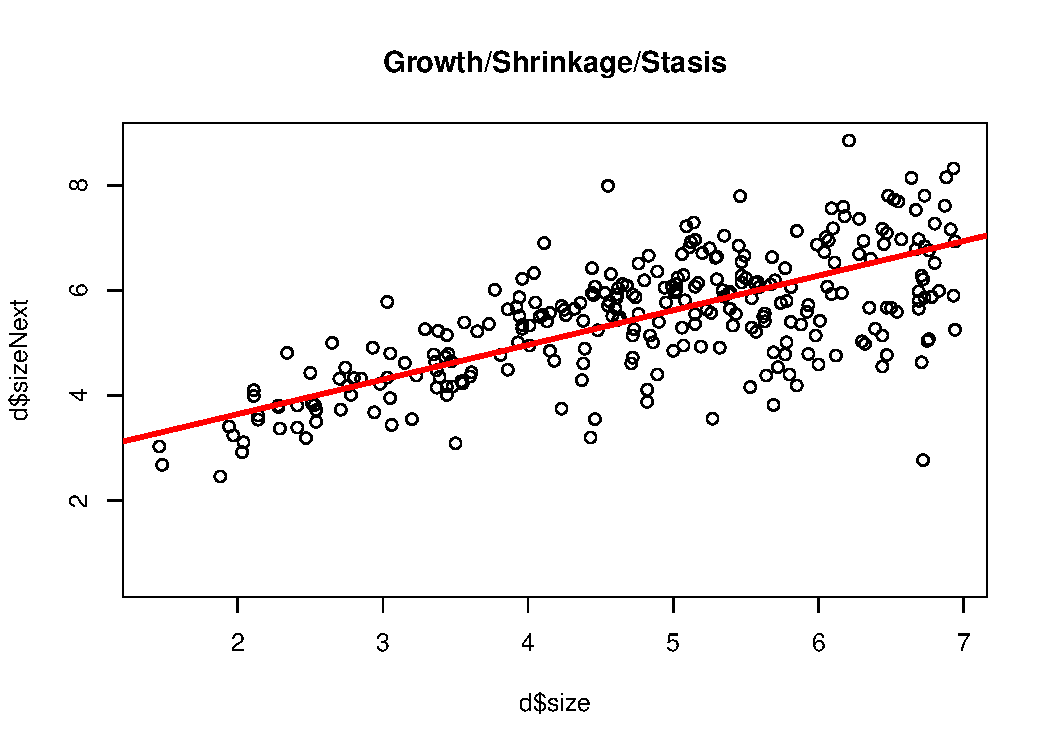
\includegraphics{IPM_Guide_Appendix_A-gls_plot}
\caption{Size dependent variance in growth.}
\label{fig:gls_plot}
\end{center}
\end{figure}

\item Modify the params data frame (where we store all the coefficients used to build the IPM) to have coefficients called growth.sd.int and growth.sd.slope and set the values of those coefficients equal to the appropriate coefficients from part (A).

\begin{Schunk}
\begin{Sinput}
 params$growth.int=coefficients(growth.reg)[1]
 params$growth.slope=coefficients(growth.reg)[2]
 params$growth.sigma2=summary(growth.reg)$sigma^2 
 params$growth.sigma2.exp=as.numeric(growth.reg$modelStruct$varStruct)
\end{Sinput}
\end{Schunk}

\item Modify the growth function, g.xy(), to allow the standard deviation argument, sd, to be a function of size. This will follow a similar pattern to the argument for mean. It's probably easiest to redefine the function g.yx() so it works with code above to create IPMs.
\begin{Schunk}
\begin{Sinput}
 g.yx=function(xp,x,params) { 			
    dnorm(xp,mean=params$growth.int+params$growth.slope*x, 
      sd=sqrt(params$growth.sigma2*exp(2*params$growth.sigma2.exp*x)))
  }
\end{Sinput}
\end{Schunk}

\item Rerun the code from sections ~\ref{sec:Make_a_kernel} and ~\ref{sec:Basic analyses} to obtain $\lambda$,  sensitivities, elasticities, etc.
\begin{Schunk}
\begin{Sinput}
 G=h*outer(y,y,g.yx,params=params) # growth matrix
 S=s.x(y,params=params)            # survival 
 P=G                               # placeholder; redefine P on the next line
 for(i in 1:n) P[,i]=G[,i]*S[i]    # growth/survival matrix
 F=h*outer(y,y,f.yx,params=params) # reproduction matrix
 K=P+F                             # full matrix
 (lam=Re(eigen(K)$values[1]))      # new population growth rate
\end{Sinput}
\begin{Soutput}
[1] 0.980247
\end{Soutput}
\begin{Sinput}
 w.eigen=Re(eigen(K)$vectors[,1])
 stable.dist=w.eigen/sum(w.eigen) 
 v.eigen=Re(eigen(t(K))$vectors[,1])
 repro.val=v.eigen/v.eigen[1] 
 v.dot.w=sum(stable.dist*repro.val)*h
 sens=outer(repro.val,stable.dist)/v.dot.w
 elas=matrix(as.vector(sens)*as.vector(K)/lam,nrow=n)
\end{Sinput}
\end{Schunk}

We can plot these results and compare to Fig.~\ref{fig:figA3}.

\begin{figure}[H]
\begin{center}
\begin{Schunk}
\begin{Sinput}
     par(mfrow=c(2,3),mar=c(4,5,2,2)) 
     image.plot(y,y,t(K), xlab="Size (t)",ylab="Size (t+1)",
        col=topo.colors(100), main="IPM matrix")
     contour(y,y,t(K), add = TRUE, drawlabels = TRUE)
     plot(y,stable.dist,xlab="Size",type="l",main="Stable size distribution")
     plot(y,repro.val,xlab="Size",type="l",main="Reproductive values") 
     image.plot(y,y,t(elas),xlab="Size (t)",ylab="Size (t+1)",main="Elasticity")
     image.plot(y,y,t(sens),xlab="Size (t)",ylab="Size (t+1)", main="Sensitivity")
\end{Sinput}
\end{Schunk}
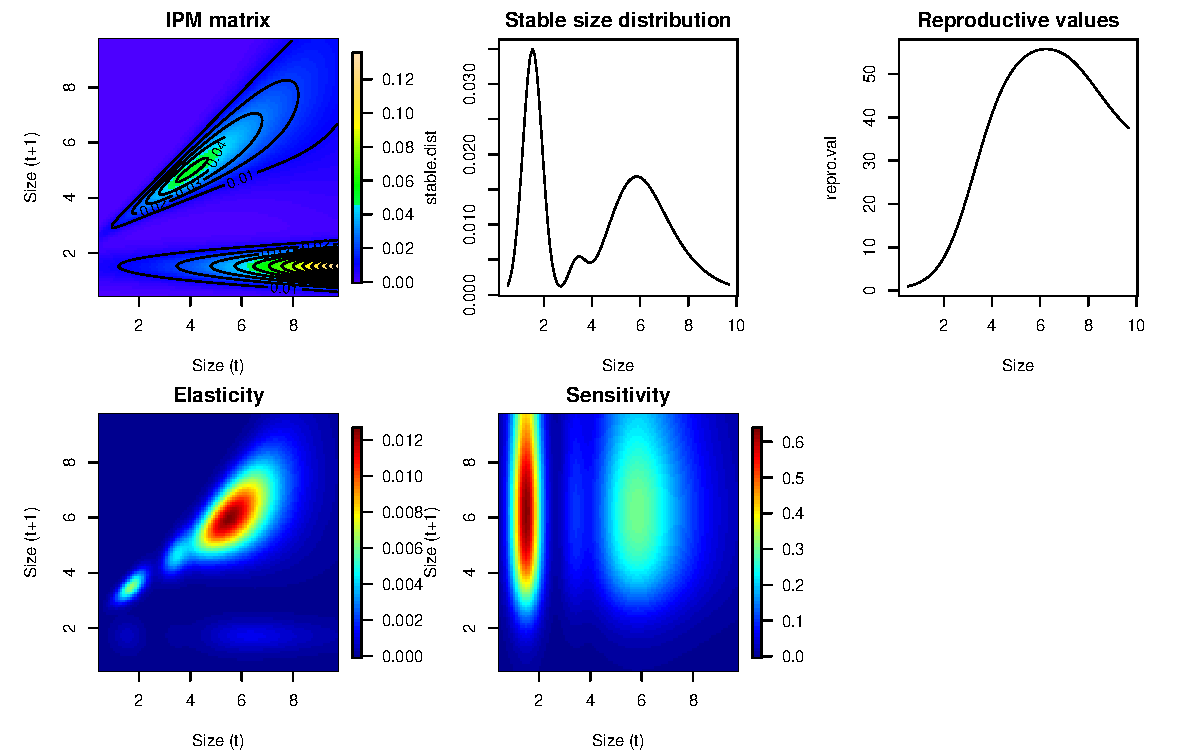
\includegraphics{IPM_Guide_Appendix_A-fig5}
\caption{Basic model output with variance in growth function modeled as a linear function of size. Compare to Fig. ~\ref{fig:figA3}.}
\label{fig:figA5}
\end{center}
\end{figure}

%TODO comment on changes

\end{enumerate}

%%%%%%%%%%%%%%%%%%%%%%%%%%%%%%%%%%%%%%%%%%%%%%%%%%%%%%%%%%%%%%%%%%%%%%%%%%%%%%
%%%%%%%%%%%%%%%%%%%%%%%%%%%%%%%%%%%%%%%%%%%%%%%%%%%%%%%%%%%%%%%%%%%%%%%%%%%%%%
\subsubsection{Eviction}
\label{sec:Eviction}
We begin by checking for unintentional eviction, wherein individuals transition beyond the size range chosen for the model, leading to inaccurate representation of the survival model (Williams et al. 2012). Because the growth function and offspring size distribution are Gaussian (Normal) probability densities, they range from -inf to +inf. Because of how we've defined the model, most of that probability for both functions falls between the minimum and maximum values of size that we've chosen for the model (0.45 and 9.735, respectively), but not all of it. If we ignore the parts of these densities that fall outside the integration limits, individuals are 'evicted from the model' and survival is incorrectly estimated (Williams et al. 2012). 

To check for eviction, we plot the survival model and the column sums of the survival/growth (P) matrix. In Fig.~\ref{fig:fig_eviction}, we see that the eviction occurs only for large individuals (size >9) because the column sums are lower than the survival models suggests that they should be.

\begin{figure}[H]
\begin{center}
\begin{Schunk}
\begin{Sinput}
     plot(y,s.x(y,params),xlab="Size",type="l",
        ylab='Survival Probability',lwd=12)
     points(y,apply(P,2,sum),col='red',lwd=3,cex=.1,pch=19) 
\end{Sinput}
\end{Schunk}
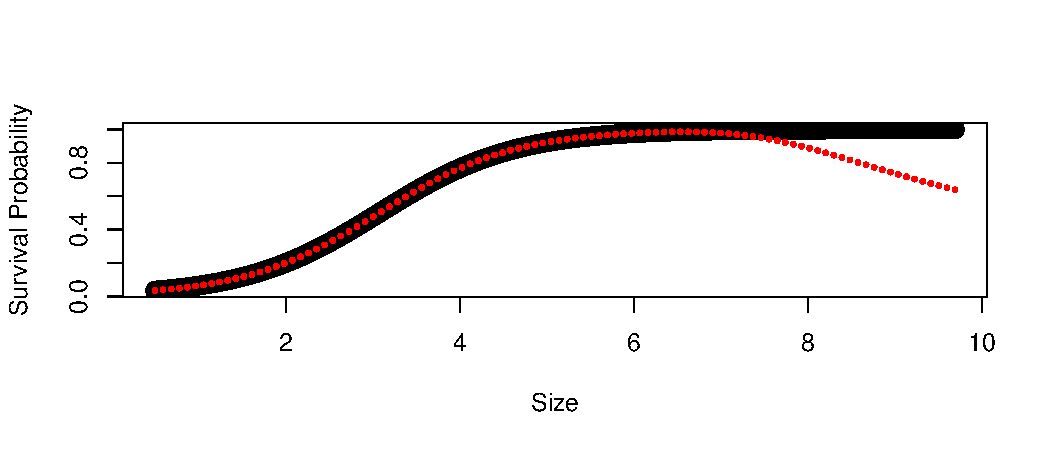
\includegraphics{IPM_Guide_Appendix_A-fig_eviction}
\caption{Comparison of predicted survival probability to observed values to test for unintentional eviction. The black line shows the fitted survival model. The red dot shows the column sums of the growth/survival matrix.}
\label{fig:fig_eviction}
\end{center}
\end{figure}

One way to correct for eviction is to return the evicted individuals to the cells at the boundaries where they were evicted. All individuals smaller than the lower integration limit are assigned to the smallest size class. This mainly affects the offspring size distribution; it sets a lower limit on offspring size. (Eviction at small sizes doesn't really affect the present model, but we mention it for completeness.) Similarly, all individuals larger than the upper integration limit can be assigned to the largest size class. This mainly affects the growth function, when individuals in the largest size class are still able to grow. A variety of approaches for correcting eviction are discussed and compared in (Williams et al. 2012).

To apply this approach, we need to modify the growth matrix before combining the growth/survival and fecundity matrices. In the following modification of the code to construct the matrix there are two loops: one that corrects for eviction of offspring and one that corrects for eviction of large adults.

\begin{Schunk}
\begin{Sinput}
 G=h*outer(y,y,g.yx,params=params) # growth matrix
 S=s.x(y,params=params) 
 P=G
   # fix eviction of offspring
 for(i in 1:(n/2)) { 
    G[1,i]<-G[1,i]+1-sum(G[,i])
    P[,i]<-G[,i]*S[i] 
  }
   # fix eviction of large adults
 for(i in (n/2+1):n) { 
    G[n,i]<-G[n,i]+1-sum(G[,i])
    P[,i]<-G[,i]*S[i] 
  }
 F=h*outer(y,y,f.yx,params=params) # reproduction matrix
 K=P+F                             # full matrix
 (lam=Re(eigen(K)$values[1]))      # new population growth rate
\end{Sinput}
\begin{Soutput}
[1] 1.013069
\end{Soutput}
\end{Schunk}

We can re-plot the columns sums to check that this solution worked. 

\begin{figure}[H]
\begin{center}
\begin{Schunk}
\begin{Sinput}
     plot(y,s.x(y,params),xlab="Size",type="l",
        ylab='Survival Probability',lwd=12)
     points(y,apply(P,2,sum),col='red',lwd=3,cex=.1,pch=19) 
\end{Sinput}
\end{Schunk}
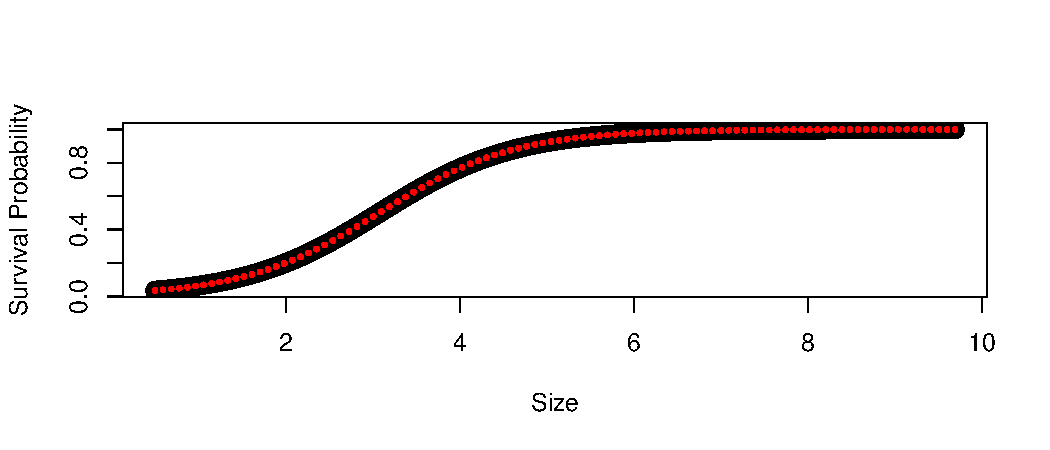
\includegraphics{IPM_Guide_Appendix_A-fig_eviction_fix}
\caption{Comparison of predicted survival probability to observed values to test for unintentional eviction after using the ceiling approach to remove eviction. The black line shows the fitted survival model. The red dot shows the column sums of the growth/survival matrix.}
\label{fig:fig_eviction_fix}
\end{center}
\end{figure}

%%%%%%%%%%%%%%%%%%%%%%%%%%%%%%%%%%%%%%%%%%%%%%%%%%%%%%%%%%%%%%%%%%%%%%%%%%%%%%
%%%%%%%%%%%%%%%%%%%%%%%%%%%%%%%%%%%%%%%%%%%%%%%%%%%%%%%%%%%%%%%%%%%%%%%%%%%%%%

\subsubsection{Quadratic Growth Function}
\label{subsec:Quadratic Growth}

The next improvement to the IPM is to add a quadratic term to the growth regression to capture the slight downward curving pattern in growth (Fig. ~\ref{fig:figA2}).  To tell the growth regression to use a quadratic term, use I(size \^ 2) as a predictor variable. For simplicity, we keep the size dependence of the growth variance from the previous section in the model, but note that we rerun the variance regressions since the residuals will change when the quadratic term is added to the model.
\begin{Schunk}
\begin{Sinput}
 growth.reg=gls(sizeNext~size+I(size^2),weights=varExp(), na.action=na.omit, data=d)
 summary(growth.reg)
\end{Sinput}
\begin{Soutput}
Generalized least squares fit by REML
  Model: sizeNext ~ size + I(size^2) 
  Data: d 
       AIC      BIC    logLik
  698.7273 716.8474 -344.3636

Variance function:
 Structure: Exponential of variance covariate
 Formula: ~fitted(.) 
 Parameter estimates:
    expon 
0.3526462 

Coefficients:
                 Value Std.Error   t-value p-value
(Intercept)  0.7802238 0.3208072  2.432065  0.0156
size         1.4981985 0.1704046  8.792009  0.0000
I(size^2)   -0.1007464 0.0204990 -4.914706  0.0000

 Correlation: 
          (Intr) size  
size      -0.972       
I(size^2)  0.925 -0.985

Standardized residuals:
        Min          Q1         Med          Q3         Max 
-3.26750298 -0.63630063  0.06390183  0.62856672  3.02974171 

Residual standard error: 0.11715 
Degrees of freedom: 280 total; 277 residual
\end{Soutput}
\begin{Sinput}
 params$growth.int=coefficients(growth.reg)[1]
 params$growth.slope=coefficients(growth.reg)[2]
 params$growth.sqrd=coefficients(growth.reg)[3]
 params$growth.sigma2=summary(growth.reg)$sigma^2 
 params$growth.sigma2.exp=as.numeric(growth.reg$modelStruct$varStruct)  
 g.yx=function(xp,x,params) { 			
    dnorm(xp,
      mean=params$growth.int+params$growth.slope*x+params$growth.sqrd*x^2,
      sd=sqrt(params$growth.sigma2*exp(2*params$growth.sigma2.exp*x)))
  }
 
\end{Sinput}
\end{Schunk}
We rerun the code to build the matrix and obtain $\lambda$, sensitivities, elasticities, etc. 
\begin{Schunk}
\begin{Sinput}
 G=h*outer(y,y,g.yx,params=params) # growth matrix
 S=s.x(y,params=params)            # survival 
 P=G                               # placeholder; redefine P on the next line
   # fix eviction of offspring
 for(i in 1:(n/2)) { 
    G[1,i]<-G[1,i]+1-sum(G[,i])
    P[,i]<-G[,i]*S[i] 
  }
   # fix eviction of large adults
 for(i in (n/2+1):n) { 
    G[n,i]<-G[n,i]+1-sum(G[,i])
    P[,i]<-G[,i]*S[i] 
  }
 #for(i in 1:n) P[,i]=G[,i]*S[i]    # growth/survival matrix
 F=h*outer(y,y,f.yx,params=params) # reproduction matrix
 K=P+F                             # full matrix
 (lam=Re(eigen(K)$values[1]))      # new population growth rate
\end{Sinput}
\begin{Soutput}
[1] 0.9835344
\end{Soutput}
\begin{Sinput}
 w.eigen=Re(eigen(K)$vectors[,1])
 stable.dist=w.eigen/sum(w.eigen) 
 v.eigen=Re(eigen(t(K))$vectors[,1])
 repro.val=v.eigen/v.eigen[1] 
 v.dot.w=sum(stable.dist*repro.val)*h
 sens=outer(repro.val,stable.dist)/v.dot.w
 elas=matrix(as.vector(sens)*as.vector(K)/lam,nrow=n)
\end{Sinput}
\end{Schunk}

We can plot these results and compare to Figs.~\ref{fig:figA3} and ~\ref{fig:figA5}. Compared to the model in Fig.~\ref{fig:figA5}, the ridge in the matrix corresponding to growth in Fig.~\ref{fig:figA6} now has a parabolic shape. The new model prevents individuals from growing continuously and sets an (asymptotic) upper limit on size where the growth regression crosses the 1:1 line. Because individuals can not growth continuously in the model in Fig.~\ref{fig:figA6}, there is now more mass in the 'adult' portion of the stable stage distribution (sizes > 4), because there are no longer very large individuals in the population, who previously were producing a very large number of offspring in the model in Fig.~\ref{fig:figA5}. Not surprisingly, there is slightly greater sensitivity/elasticity to survival of individuals reaching sizes near 6, corresponding to the largest individuals in current model. 

\begin{figure}[H]
\begin{center}
\begin{Schunk}
\begin{Sinput}
     par(mfrow=c(2,3),mar=c(4,5,2,2)) 
     image.plot(y,y,t(K), xlab="Size (t)",ylab="Size (t+1)",
        col=topo.colors(100), main="IPM matrix")
     contour(y,y,t(K), add = TRUE, drawlabels = TRUE)
     plot(y,stable.dist,xlab="Size",type="l",main="Stable size distribution")
     plot(y,repro.val,xlab="Size",type="l",main="Reproductive values") 
     image.plot(y,y,t(elas),xlab="Size (t)",ylab="Size (t+1)",main="Elasticity")
     image.plot(y,y,t(sens),xlab="Size (t)",ylab="Size (t+1)", main="Sensitivity")
\end{Sinput}
\end{Schunk}
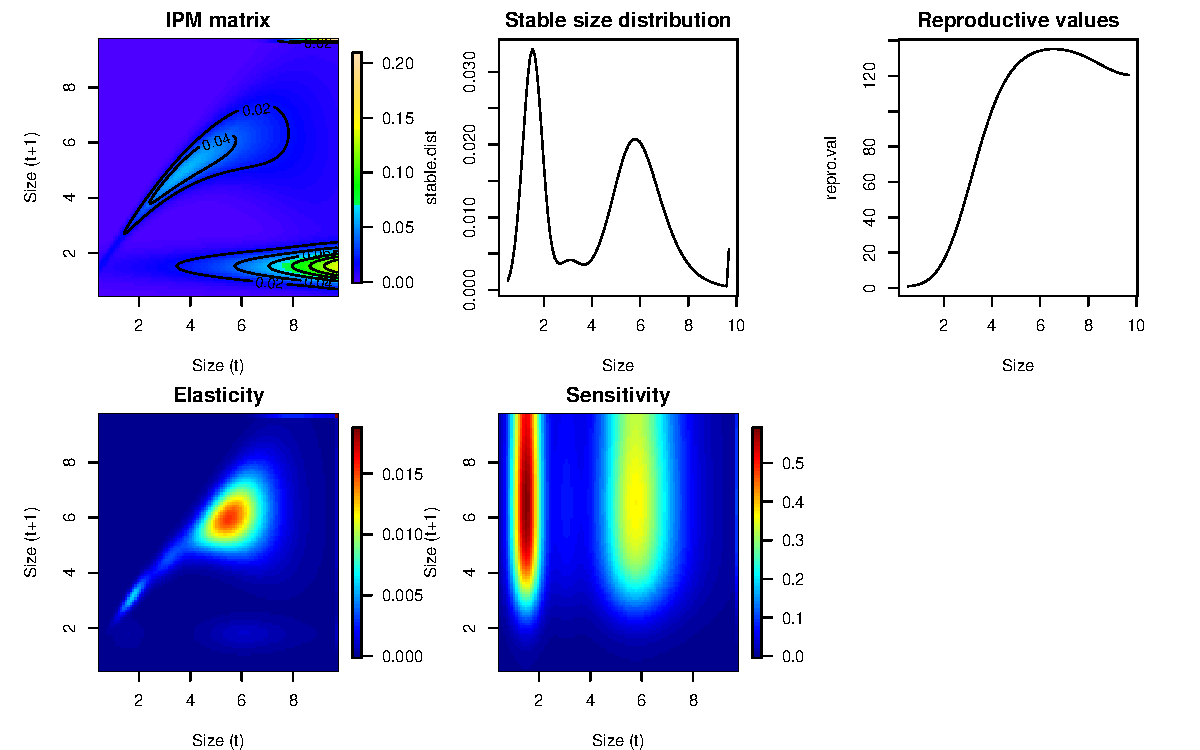
\includegraphics{IPM_Guide_Appendix_A-fig6}
\caption{Basic model output with quadratic term in growth function. Compare to Figs.~\ref{fig:figA3}, ~\ref{fig:figA5}.}
\label{fig:figA6}
\end{center}
\end{figure}
  
%%%%%%%%%%%%%%%%%%%%%%%%%%%%%%%%%%%%%%%%%%%%%%%%%%%%%%%%%%%%%%%%%%%%%%%%%%%%%%
%%%%%%%%%%%%%%%%%%%%%%%%%%%%%%%%%%%%%%%%%%%%%%%%%%%%%%%%%%%%%%%%%%%%%%%%%%%%%%

\subsubsection{Flowering Probability}
\label{subsec:Flowering Probability}

The final improvement to the IPM is to incorporate a model for flowering probability. There are two issues in play here. One is that we know the biology and expect larger individuals to flower more. The other is that the data don't support the form of the original model. More generally, it is not a good idea to combine multiple processes into a single function, as this makes it hard to model the data. Consider the case where the plant does not flower each year, perhaps dependent on stress deriving from some environmental factor. We expect that larger plants are more likely to flower because they can maintain a sufficient amount of stored resources to buffer against environmental variation. We might not know what triggers the decision to flower, but we can at least describe its size dependence by including the probability of flowering in the model. The flowering probability function will enter the reproduction kernel (called f.xy()), defined in section ~\ref{sec:Define functions to describe life history}. The version of f.xy() used above simply assumes that all plants flower, so including the flowering probability function will reduce this number. (Alternatively, one could use a zero-inflated model, but since we have information on flowering, it is preferable to split up the distinct processes of flowering and reproductive output conditional on flowering.)  Including a flowering probability model requires 5 steps:
	 
\begin{enumerate}[(A)]
\item First, we write the flowering probability function. Flowering probability is most easily modeled using logistic regression, so this will be very similar to the survival function (s.xy) above. Call the function p.flower.x(). and store the slope and intercept of the flowering regression as params$flower.int and param$flower.slope, respectively, which are defined below.
\begin{Schunk}
\begin{Sinput}
 p.flower.x=function(x,params) {
  	u=exp(params$flower.int+params$flower.slope*x)
  	return(u/(1+u))
  }
\end{Sinput}
\end{Schunk}

\item Next, we modify the reproduction function (f.xy) to include the flowering probability function. This just amounts to multiplying the argument in f.xy by p.flower.x. 
\begin{Schunk}
\begin{Sinput}
 f.yx=function(xp,x,params) { 		
    p.flower.x(x,params)* 
  	params$establishment.prob*
  	dnorm(xp,mean=params$recruit.size.mean,sd=params$recruit.size.sd)*
  	exp(params$seed.int+params$seed.slope*x)
  }
\end{Sinput}
\end{Schunk}

\item Now, we fit a logistic regression for flowering probability. See the data frame for binary flowering data under d\$fec.flower. From this regression, we obtain a slope and intercept, and store these in the param vector.  

\begin{Schunk}
\begin{Sinput}
 flower.reg=glm(fec.flower~size,data=d,family=binomial())
 summary(flower.reg)
\end{Sinput}
\begin{Soutput}
Call:
glm(formula = fec.flower ~ size, family = binomial(), data = d)

Deviance Residuals: 
     Min        1Q    Median        3Q       Max  
-2.90763   0.05881   0.16048   0.39906   1.94232  

Coefficients:
            Estimate Std. Error z value Pr(>|z|)    
(Intercept)  -6.5495     0.9564  -6.848 7.48e-12 ***
size          1.9081     0.2465   7.740 9.92e-15 ***
---
Signif. codes:  
0 ‘***’ 0.001 ‘**’ 0.01 ‘*’ 0.05 ‘.’ 0.1 ‘ ’ 1

(Dispersion parameter for binomial family taken to be 1)

    Null deviance: 285.68  on 279  degrees of freedom
Residual deviance: 144.30  on 278  degrees of freedom
  (220 observations deleted due to missingness)
AIC: 148.3

Number of Fisher Scoring iterations: 6
\end{Soutput}
\begin{Sinput}
 params$flower.int=coefficients(flower.reg)[1]
 params$flower.slope=coefficients(flower.reg)[2]
\end{Sinput}
\end{Schunk}
\item Update the regression for seed number to include only the individuals that flowered.

\begin{Schunk}
\begin{Sinput}
 seed.reg=glm(fec.seed~size,data=d[d$fec.flower==1,],family=poisson())
 summary(seed.reg)
\end{Sinput}
\begin{Soutput}
Call:
glm(formula = fec.seed ~ size, family = poisson(), data = d[d$fec.flower == 
    1, ])

Deviance Residuals: 
     Min        1Q    Median        3Q       Max  
-2.54532  -0.76716   0.03013   0.66809   2.98617  

Coefficients:
            Estimate Std. Error z value Pr(>|z|)    
(Intercept)  2.85617    0.07447  38.353  < 2e-16 ***
size         0.05076    0.01370   3.706  0.00021 ***
---
Signif. codes:  
0 ‘***’ 0.001 ‘**’ 0.01 ‘*’ 0.05 ‘.’ 0.1 ‘ ’ 1

(Dispersion parameter for poisson family taken to be 1)

    Null deviance: 250.71  on 221  degrees of freedom
Residual deviance: 236.90  on 220  degrees of freedom
  (220 observations deleted due to missingness)
AIC: 1339

Number of Fisher Scoring iterations: 4
\end{Soutput}
\begin{Sinput}
 params$seed.int=coefficients(seed.reg)[1]
 params$seed.slope=coefficients(seed.reg)[2]
\end{Sinput}
\end{Schunk}

\item Finally, we rerun the code from sections ~\ref{sec:Make_a_kernel} and ~\ref{sec:Basic analyses} to obtain $\lambda$, sensitivities, elasticities, etc., and plot the results. 
\begin{Schunk}
\begin{Sinput}
 G=h*outer(y,y,g.yx,params=params) # growth matrix
 S=s.x(y,params=params)            # survival 
 P=G                               # placeholder; redefine P on the next line
   # fix eviction of offspring
 for(i in 1:(n/2)) { 
    G[1,i]<-G[1,i]+1-sum(G[,i])
    P[,i]<-G[,i]*S[i] 
  }
   # fix eviction of large adults
 for(i in (n/2+1):n) { 
    G[n,i]<-G[n,i]+1-sum(G[,i])
    P[,i]<-G[,i]*S[i] 
  }
 # for(i in 1:n) P[,i]=G[,i]*S[i]    # growth/survival matrix
 F=h*outer(y,y,f.yx,params=params) # reproduction matrix
 K=P+F                             # full matrix
 (lam=Re(eigen(K)$values[1]))      # new population growth rate
\end{Sinput}
\begin{Soutput}
[1] 0.9765733
\end{Soutput}
\begin{Sinput}
 w.eigen=Re(eigen(K)$vectors[,1])
 stable.dist=w.eigen/sum(w.eigen) 
 v.eigen=Re(eigen(t(K))$vectors[,1])
 repro.val=v.eigen/v.eigen[1] 
 v.dot.w=sum(stable.dist*repro.val)*h
 sens=outer(repro.val,stable.dist)/v.dot.w
 elas=matrix(as.vector(sens)*as.vector(K)/lam,nrow=n)
\end{Sinput}
\end{Schunk}

\begin{figure}[H]
\begin{center}
\begin{Schunk}
\begin{Sinput}
     par(mfrow=c(2,3),mar=c(4,5,2,2)) 
     image.plot(y,y,t(K), xlab="Size (t)",ylab="Size (t+1)",
        col=topo.colors(100), main="IPM matrix")
     contour(y,y,t(K), add = TRUE, drawlabels = TRUE)
     plot(y,stable.dist,xlab="Size",type="l",main="Stable size distribution")
     plot(y,repro.val,xlab="Size",type="l",main="Reproductive values") 
     image.plot(y,y,t(elas),xlab="Size (t)",ylab="Size (t+1)",main="Elasticity")
     image.plot(y,y,t(sens),xlab="Size (t)",ylab="Size (t+1)", main="Sensitivity")
     plot(y,predict(flower.reg,newdata=data.frame(size=y),type='response'),
        xlab="Size (t)", ylab="Flowering probability",type='l')
\end{Sinput}
\end{Schunk}
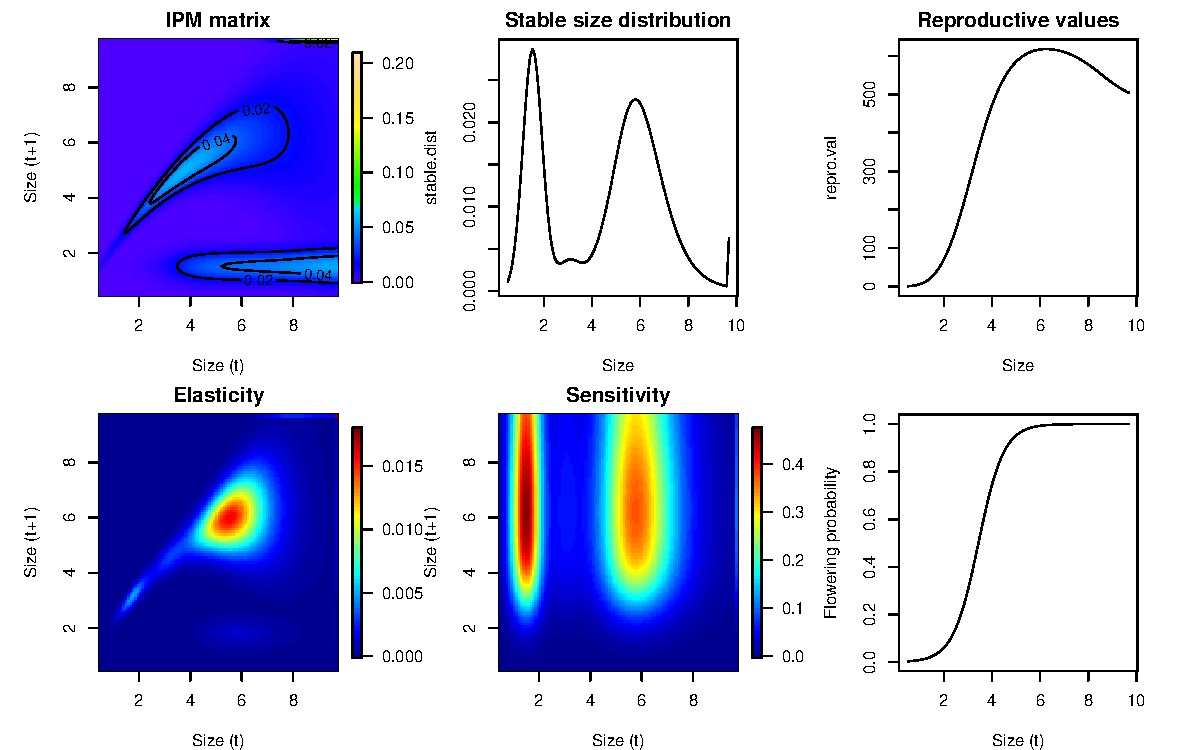
\includegraphics{IPM_Guide_Appendix_A-fig7}
\caption{Basic model output with flowering probability function included. Compare to Figs.~\ref{fig:figA3}, ~\ref{fig:figA5}, ~\ref{fig:figA6}.}
\label{fig:figA7}
\end{center}
\end{figure}

\end{enumerate}

Note that $\lambda$ decreases slightly compared to the model in Fig.~\ref{fig:figA6}, because fewer individuals reproduce. Compared to Fig.~\ref{fig:figA6}, the peak in the matrix and sensitivity is shifted toward individuals reaching a size near 6, where the flowering probability function asymptotes to 1 (Fig.~\ref{fig:figA7}). The stable size distribution shifts toward having more mass in established individuals (size>4) compared to Fig.~\ref{fig:figA6}. In the model in Fig.~\ref{fig:figA6}, small individuals reproduced 100\% of the time; because fewer small individuals reproduce in the model in Fig.~\ref{fig:figA7}, a greater number of large individuals compensate for the lost reproductive output in the stable size distribution. 

\subsection{Diagnostics}
\label{sec:Diagnostics}

In this section, we illustrate how to calculate some of the diagnostics for the kernel discussed in Section III of the main text. For these diagnostics, we rely on the R package 'IPMpack' (Metcalf et al. 2013), which conveniently implements the necessary calculations. While appendices C-G use IPMpack for the full construction of IPMs, we illustrate here how the diagnostic tools can be used for an IPM matrix constructed outside the package. 

%%%%%%%%%%%%%%%%%%%%%%%%%%%%%%%%%%%%%%%%%%%%%%%%%%%%%%%%%%%%%%%%%%%%%%%%%%%%%%
%%%%%%%%%%%%%%%%%%%%%%%%%%%%%%%%%%%%%%%%%%%%%%%%%%%%%%%%%%%%%%%%%%%%%%%%%%%%%%

\subsubsection{Passage times}
\label{sec:Passage times}

Next, we estimate the predicted time to reach critical a life history event. We begin with the life expectancy. This requires converting the matrix to an object of class 'IPMmatrix' that IPMpack can work with. Type \emph{??IPMmatrix} for a description of the objects of class 'IPMmatrix'. 

% Ask johan about estimates of these and references.
\begin{Schunk}
\begin{Sinput}
 library(IPMpack)
 Pmat = new("IPMmatrix", nDiscrete = 0, nEnvClass = 0, 
          nBigMatrix = n, nrow = n, ncol = n, meshpoints = y, 
          env.index = 0, names.discrete = '')
 Pmat[, ] = P 
 str(Pmat)
\end{Sinput}
\begin{Soutput}
Formal class 'IPMmatrix' [package "IPMpack"] with 7 slots
  ..@ .Data         : num [1:100, 1:100] 5.74e-14 5.44e-12 3.34e-10 1.31e-08 3.32e-07 ...
  ..@ nDiscrete     : num 0
  ..@ nEnvClass     : num 0
  ..@ nBigMatrix    : num 100
  ..@ meshpoints    : num [1:100] 0.496 0.589 0.682 0.775 0.868 ...
  ..@ env.index     : num 0
  ..@ names.discrete: chr ""
\end{Soutput}
\begin{Sinput}
 (mle=meanLifeExpect(Pmat))
\end{Sinput}
\begin{Soutput}
  [1]  1.067947  1.087713  1.113730  1.147586  1.191108
  [6]  1.246350  1.315576  1.401236  1.505916  1.632291
 [11]  1.783059  1.960869  2.168249  2.407523  2.680741
 [16]  2.989599  3.335372  3.718851  4.140281  4.599314
 [21]  5.094971  5.625612  6.188933  6.781973  7.401147
 [26]  8.042312  8.700842  9.371742 10.049768 10.729571
 [31] 11.405840 12.073441 12.727552 13.363778 13.978236
 [36] 14.567625 15.129262 15.661087 16.161653 16.630089
 [41] 17.066050 17.469655 17.841420 18.182189 18.493065
 [46] 18.775347 19.030470 19.259955 19.465367 19.648272
 [51] 19.810214 19.952689 20.077125 20.184874 20.277197
 [56] 20.355265 20.420153 20.472839 20.514208 20.545050
 [61] 20.566068 20.577879 20.581016 20.575939 20.563033
 [66] 20.542615 20.514941 20.480210 20.438568 20.390116
 [71] 20.334920 20.273015 20.204418 20.129137 20.047187
 [76] 19.958598 19.863433 19.761805 19.653884 19.539914
 [81] 19.420226 19.295242 19.165478 19.031550 18.894166
 [86] 18.754116 18.612264 18.469530 18.326870 18.185258
 [91] 18.045663 17.909030 17.776258 17.648185 17.525569
 [96] 17.409079 17.299286 17.196655 17.101543 17.014202
\end{Soutput}
\end{Schunk}

Let's plot the result:

\begin{figure}[H]
\begin{center}
\begin{Schunk}
\begin{Sinput}
   plot(y,meanLifeExpect(Pmat), xlab="Size (t)",ylab="Time")
\end{Sinput}
\end{Schunk}
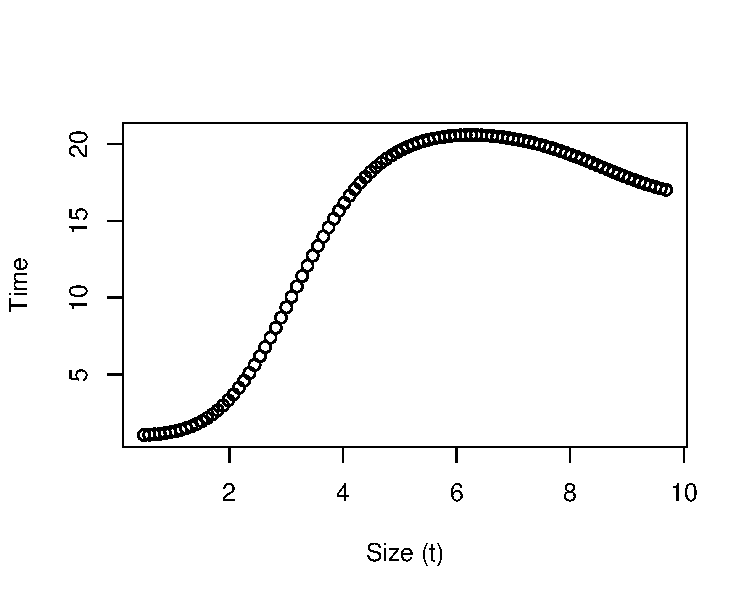
\includegraphics{IPM_Guide_Appendix_A-fig_life_expect}
\caption{Life expectancy; the predicted mean lifespan of an individual of size z at time 0.}
\label{fig:fig_life_expect}
\end{center}
\end{figure}
    
These life expectancy estimates seem reasonable for a long-lived perennial plant, so we continue to other diagnostics. One might also estimate the time to a variety of other life history events (cf. Caswell 2001, Chapter 5) to check that the model reasonably represents the species' biology.

% The passage times to the maximum size are all greater than 110 years! Although we're working with a long-lived perennial herb, this is unreasonable, so we need to revisit the survival/growth kernel to determine the source of the problem. 
% 
% % for time to first flowering
% <<>>=
% (ptf=passageTime(chosenSize=5.5, Pmat))
% 
%     plot(y,passageTime(chosenSize=1, Pmat), xlab="Size (t)",ylab="Time", main="",type='l',lwd=3)
%     sizes=c(1,2,3,4,5,6,7,8,9)  
%     #lines(y,ptf,col='red',lwd=3)
%     for (i in 1:8){
%       lines(y,passageTime(chosenSize=sizes[i], Pmat),lwd=i)
%     }
% @

% Such passage times are not reasonable for an herb, nor is an asymptotic size of 6, since many individuals have been observed at larger sizes in the data set (Fig.~\ref{fig:figA1}). One way to resolve this is to remove the quadtratic term (added in ~\ref{subsec:Quadratic Growth}) from the growth model. This is case where biological sensibility must supercede statistical fit: although the quadratic model fits the growth data slightly better, it produces biologically unrealistic results. More flexible regression models are possible (Appendix D), but for simplicity we'll revert back to the simpler growth model that omits the quadratic term. The code below rebuilds the linear model, corrects for eviction, and calculates the passsage time, which is now more biologically reasonable. Note that eviction is more prevalent when using the simpler growth model because individuals can readily grow to larger sizes. 
% 
% <<>>=
%   # original growth model
% growth.reg=lm(sizeNext~size,data=d)
% params$growth.int=coefficients(growth.reg)[1]
% params$growth.slope=coefficients(growth.reg)[2]
%   # variance in growth
% growth.sd.reg=lm(abs(resid(growth.reg))~growth.reg$model$size)
% params$growth.sd.int=coefficients(growth.sd.reg)[1]
% params$growth.sd.slope=coefficients(growth.sd.reg)[2] 
%   # growth density function
% g.yx=function(xp,x,params) {   		
% 	dnorm(xp,mean=params$growth.int+params$growth.slope*x, 
%     sd=params$growth.sd.int+params$growth.sd.slope*x)
% }
%   # construct kernel
% G=h*outer(y,y,g.yx,params=params) # growth kernel
% S=s.x(y,params=params)            # survival 
% P=G                               # placeholder; redefine P on the next line
%   # fix eviction
% for(i in 1:(n/2)) { 
%   G[1,i]<-G[1,i]+1-sum(G[,i])
%   P[,i]<-G[,i]*S[i] 
% }
% for(i in (n/2+1):n) { 
%   G[n,i]<-G[n,i]+1-sum(G[,i])
%   P[,i]<-G[,i]*S[i] 
% }
% F=h*outer(y,y,f.yx,params=params) # reproduction kernel
% K=P+F                             # full kernel
% (lam=Re(eigen(K)$values[1]))      # new population growth rate
% Pmat[, ] = P 
% (passageTime(chosenSize=max.size, Pmat))
% 
% @

%%%%%%%%%%%%%%%%%%%%%%%%%%%%%%%%%%%%%%%%%%%%%%%%%%%%%%%%%%%%%%%%%%%%%%%%%%%%%%
%%%%%%%%%%%%%%%%%%%%%%%%%%%%%%%%%%%%%%%%%%%%%%%%%%%%%%%%%%%%%%%%%%%%%%%%%%%%%%

\subsubsection{Maximum size}
\label{sec:Maximum size}

The mean of the growth function crosses the 1:1 line in Fig.~\ref{fig:fig_kernel1to1} around size = 6, this sets an \emph{approximate} upper bound on the size to which individuals can grow. For example, if an individual is size 8 at time \emph{t}, the expectation from this model is that it will be size 6.2 at time \emph{t+1}. There's a small chance that it could grow to be larger than size 8, since the matrix has a nonzero values above the 1:1 line at size(t) = 8, but this is very unlikely. Since individuals larger than size 6 tend to shrink back toward size 6, we would expect that it should take a very long time to observe growth over a few consecutive years to reach the maximum size in the model (9.6). This illustrates why it can be valuable to compare the growth model to the 1:1 line: where the mean of the growth model intersects 1:1 sets the approximate asymptotic size on individuals (Section III.A in the main text). This seems reasonable given the distribution of observed sizes shown in Fig.~\ref{fig:fig_kernel1to1}; most individuals are around size 6 while just a few grow to larger sizes. Note that if mortality is high, a species is slow growing, or the environment is variable, individuals may not reach this modeled maximum size.

\begin{figure}[H]
\begin{center}
\begin{Schunk}
\begin{Sinput}
     par(mfrow=c(2,1),mar=c(4,5,2,2))    
     image.plot(y,y,t(P), xlab="Size (t)",ylab="Size (t+1)",
        col=topo.colors(100), main="IPM matrix")
     contour(y,y,t(P), add = TRUE, drawlabels = TRUE)
     abline(0,1,lwd=3,lty=2)
     plot(density(d$sizeNext[!is.na(d$sizeNext)]),xlab='Size(t+1)',
        main='Observed distribution of sizes')
\end{Sinput}
\end{Schunk}
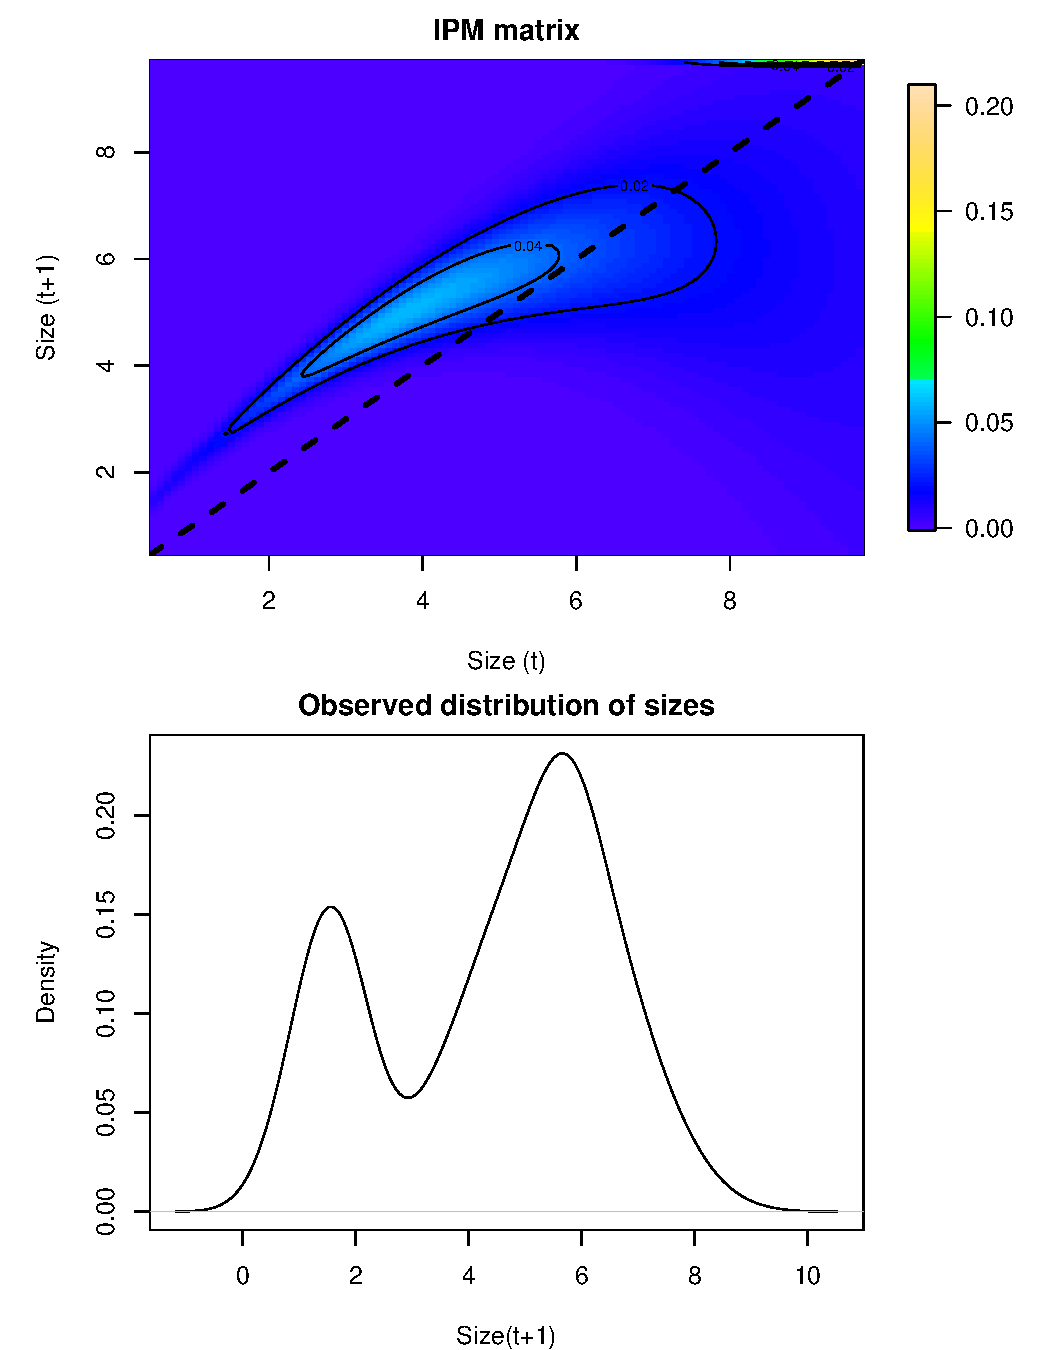
\includegraphics{IPM_Guide_Appendix_A-fig_kernel1to1}
\caption{matrix with 1:1 line overlayed (dashed black line).}
\label{fig:fig_kernel1to1}
\end{center}
\end{figure}

%%%%%%%%%%%%%%%%%%%%%%%%%%%%%%%%%%%%%%%%%%%%%%%%%%%%%%%%%%%%%%%%%%%%%%%%%%%%%%
%%%%%%%%%%%%%%%%%%%%%%%%%%%%%%%%%%%%%%%%%%%%%%%%%%%%%%%%%%%%%%%%%%%%%%%%%%%%%%

\subsubsection{Transient Dynamics}
\label{sec:Transient Dynamics}
Transient dynamics can be important if the population size structure is not near the stable size distribution. If interest lies in short term projections, considering transient dynamics may be particularly important for accurate predictions. Below we compare the asymptotic population growth rate to the inter-annual estimates to determine the time needed to reach a steady state. In this case, it requires only a few time steps, which means that the asymptotic predictions are sufficient for describing dynamics beyond a few years. The time scale for reaching the steady state can be estimated from the damping ratio (Caswell 2001, p. 95): the ratio of the dominant eigenvalue to the second largest one. Small values (near 1) mean slow transients; higher values means the dominant eigenvalue dictates the dynamics.

\begin{Schunk}
\begin{Sinput}
 (lam=Re(eigen(K)$values[1]))      # asymptotic growth rate
\end{Sinput}
\begin{Soutput}
[1] 0.9765733
\end{Soutput}
\begin{Sinput}
 (damp=Re(eigen(K)$values[1])/Re(eigen(K)$values[2])) # damping ratio
\end{Sinput}
\begin{Soutput}
[1] 3.892877
\end{Soutput}
\begin{Sinput}
 initial.pop=runif(100)  #random starting population structure
 initial.pop=initial.pop/sum(initial.pop)
 nyears=20
 size.dist=matrix(NA,n,nyears)
 lambda=rep(NA,nyears)
 xold=initial.pop
 for(i in 1:nyears){
  	xnew=K%*%xold
    lambda[i]=sum(xnew)/sum(xold)
  	size.dist[,i]=xnew
    xold=xnew
  }
 lambda
\end{Sinput}
\begin{Soutput}
 [1] 1.0269669 0.9471916 0.9645584 0.9739331 0.9763776
 [6] 0.9767083 0.9766618 0.9766058 0.9765812 0.9765741
[11] 0.9765729 0.9765730 0.9765732 0.9765733 0.9765733
[16] 0.9765733 0.9765733 0.9765733 0.9765733 0.9765733
\end{Soutput}
\begin{Sinput}
 (mean.lam=exp(mean(log(lambda))))
\end{Sinput}
\begin{Soutput}
[1] 0.9768053
\end{Soutput}
\begin{Sinput}
 
\end{Sinput}
\end{Schunk}
Note that the mean value of $\lambda$ will be different than the asymptotic value during a period where transient dynamics are important. 

%%%%%%%%%%%%%%%%%%%%%%%%%%%%%%%%%%%%%%%%%%%%%%%%%%%%%%%%%%%%%%%%%%%%%%%%%%%%%%
%%%%%%%%%%%%%%%%%%%%%%%%%%%%%%%%%%%%%%%%%%%%%%%%%%%%%%%%%%%%%%%%%%%%%%%%%%%%%%

\section{Conclusions}

Using this appendix as a guide, modelers should be able to construct basic stage structured IPMs from scratch. In appendices C-F, we illustrate how components of this process can automated using the R package IPMpack (Metcalf et al. 2013). For other examples of models  similar to the one presented here, see Yule et al. (2013); Miller et al. 2009; Wallace et al. 2012 (crocodiles, though with similar vital rate models). 

This appendix illustrates the common procedure of iteratively refining an IPM to capture greater complexity in vital rates. Many further refinements are possible. For example, one might wish to use more flexible forms of regression to accommodate nonlinear responses of vital rates (see Appendix G). Or, one might wish to include covariates, such as environmental predictors, that further refine predictive power of the vital rate regressions (see Appendix B). A more complex description of fecundity might also be desirable to disentangle the various processes that lead seed loss (see Appendix B; C).

%%%%%%%%%%%%%%%%%%%%%%%%%%%%%%%%%%%%%%%%%%%%%%%%%%%%%%%%%%%%%%%%%%%%%%%%%%%%%%
%%%%%%%%%%%%%%%%%%%%%%%%%%%%%%%%%%%%%%%%%%%%%%%%%%%%%%%%%%%%%%%%%%%%%%%%%%%%%%

\section{Acknowledgements}
Some of the code has been adapted from Nicole et al. (2011). 

\section{References}
\begin{itemize}

\item Caswell, H. (2001). Matrix population models: construction, analysis, and interpretation. Sinauer, Sunderland, MA.

\item Metcalf, C., McMahon, S.M., Salguero-Gomez, R. \& Jongejans, E. (2013). IPMpack: an R package for integral projection models. Methods in Ecology and Evolution, 4, 195-200.

\item Miller, T.E.X., Louda, S.M., Rose, K.A. \& Eckberg, J.O. (2009). Impacts of insect herbivory on cactus population dynamics: experimental demography across an environmental gradient. Ecological Monographs, 79, 155-172.

\item Nicole, F., Dahlgren, J.P., Vivat, A., Till-Bottraud, I. \& Ehrlen, J. (2011). Interdependent effects of habitat quality and climate on population growth of an endangered plant. Journal of Ecology, 99, 1211-1218.

\item Wallace, K., Leslie, A. \& Coulson, T. (2012). Re-evaluating the effect of harvesting regimes on Nile crocodiles using an integral projection model (M. Boots, Ed.). Journal of Animal Ecology, 82, 155-165.

\item Williams, J.L., Miller, T.E.X \& Ellner, S.P. (2012). Avoiding unintentional eviction from integral projection models. Ecology, 93, 2008-2014.

\item Yule, K.M., Miller, T.E.X. \& Rudgers, J.A. (2013). Costs, benefits, and loss of vertically transmitted symbionts affect host population dynamics. Oikos, in press.

\end{itemize}


\end{document}










